\cleardoublepage

\chapter{Wprowadzenie do generowania wspomaganego wyszukiwaniem}
W celu zapewnienia modelowi aktualnego stanu wiedzy lub dostępu do naszych prywatnych zasobów danych istnieje znacznie bardziej wydajne podejście niż fine-tuning. Chodzi o technikę RAG, którą ze szczegółami przybliżono w niniejszym rozdziale. Dodatkowo, autor pochylił się nad definicją agentów AI, które w doskonały sposób implementują tę technikę. 


    \section{Definicja techniki RAG}
    Generowanie wspomagane wyszukiwaniem (ang. \textit{retrieval-augmented generation} — RAG) jest techniką umożliwiającą dużym modelom językowym pozyskiwanie i przetwarzanie nowych informacji z zewnętrznych źródeł danych bez konieczności modyfikowania tych modeli. Pozwala to chatbotom zredukować halucynacje i zapewnić bardziej dokładne odpowiedzi na pytania dotyczące źródeł danych, na których model nie został wytrenowany. Mogą to być dane zarówno ustrukturyzowane jak i nieustrukturyzowane, takie jak: bazy danych SQL, prywatne pliki PDF, strony internetowe czy repozytoria kodu. Dzięki temu rozwiązaniu, można zapewnić chatbotom stały dostęp do aktualnej wiedzy ze świata, co pozwala zniwelować ograniczenia wynikające z daty zakończenia treningu modelu. Jedną z kluczowych zalet podejścia RAG jest zdolność LLMa do podawania źródeł danych, a nawet cytowania konkretnego fragmentu w swojej wypowiedzi. Pozwala to użytkownikom weryfikować informacje oraz zwiększyć zaufanie do generowanej przez model treści \cite{llm_for_production2024}. Na ilustracji \ref{rag} pokazano w uproszczeniu jak działa RAG.

    \begin{center}
        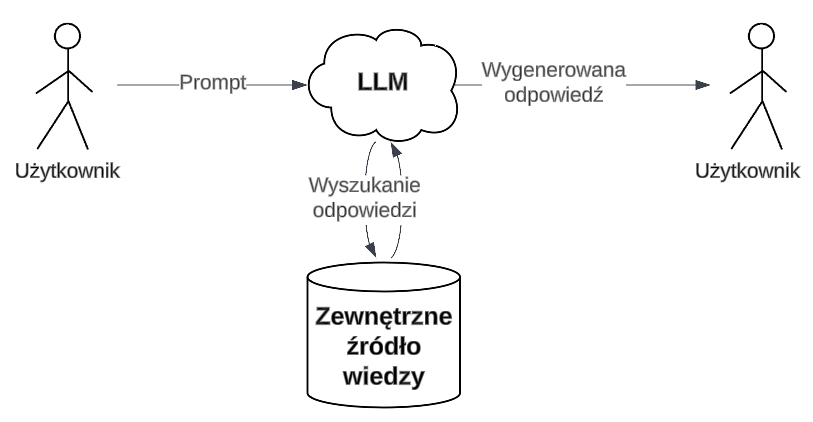
\includegraphics[width=0.6\textwidth]{rysunki/rag.png}
        \captionof{figure}{Uproszczony schemat generowania wspomaganego wyszukiwaniem}
        \label{rag}
    \end{center}
        
        
        \subsection{Embedder i wektorowa baza danych}
        Embedder przekształca zawartość źródła danych w reprezentację wektorową (embeddingi). Natomiast, wektorowa baza danych, która w większości przypadków stanowi zewnętrzne źródło wiedzy, przechowuje te embeddingi wraz z metadanymi dotyczącymi tekstów, obrazów czy audio. Pozwala to wnieść dodatkowy kontekst, czyli informacje z zewnętrznych źródeł danych do LLMa, który je wyszukuje na podstawie podobieństwa semantycznego do zapytania użytkownika. Warto nadmienić, że zawartość przetwarzanego dokumentu należy wpierw podzielić na wiele mniejszych porcji (ang. \textit{chunking}). Dodatkowo wyznacza się wspólne części kolejnych porcji tekstu (ang. \textit{overlapping}), w celu zachowania kontekstu między fragmentami. Standardowy rozmiar chunka wynosi od 256 do 512 tokenów, natomiast wartość overlapu zawiera się między 50 a 100 tokenów.
        
        
        \subsection{Wydobywanie informacji i generowanie odpowiedzi}
        Do szukania oraz pozyskiwania odpowiednich dokumentów i faktów z zewnętrznej bazy danych służy retriever. Podczas wydobywania informacji, nieustrukturyzowane zapytanie (prompt) użytkownika przekształcane jest na odpowiednią przestrzeń wektorową w celu odnalezienia istotnych informacji z bazy wektorowej. Następnie, generator analizuje pozyskaną treść i dopasowuje ją do zapytania użytkownika. Z wykorzystaniem dużego modelu językowego, tworzy odpowiedź w języku naturalnym uwzględniając wyekstrahowane fakty.


        \subsection{Porównanie RAG i fine-tuningu}
        Różnica między podejściem RAG i fine-tuning polega na tym, że te pierwsze poszerza wiedzę modelu \enquote{podłączając} go do własnej bazy danych, kiedy drugie wiąże się z kosztownym poszerzeniem wyuczonej już wiedzy modelu w konkretnej dziedzinie. Nie można jednogłośnie określić, które rozwiązanie jest lepsze, gdyż oba mają swoje zalety i wady, a dobór podejścia jest zależny od celu jaki chce się osiągnąć. RAG i fine-tuning nie wykluczają się wzajemnie, lecz mogą się uzupełniać, podnosząc wydajność modelu w określonych obszarach kompetencji modelu. W poniższej tabeli \ref{rag_vs_finetuning}, na podstawie artykułu \cite{rag_for_llm2023}, przedstawiono porównanie tych dwóch podejść.

        \begin{table}[h]
            \centering
            \caption{Zestawienie RAG i fine-tuningu \cite{rag_for_llm2023}}
            \begin{tabularx}{\textwidth}{|p{3.5cm}|X|X|}
            \hline
            \textbf{Porównywana cecha} & \textbf{RAG} & \textbf{Fine-tuning} \\
            \hline
            Aktualizacja wiedzy & Umożliwia bezpośrednią aktualizację bazy wiedzy, zapewniając stałą aktualność informacji bez konieczności dotrenowania modelu, co jest odpowiednie dla dynamicznie zmieniających się danych. & Statyczna wiedza modelu utrwalona w jego parametrach. Wymagane jest dotrenowanie w celu aktualizacji stanu wiedzy. \\ \hline
            
            Przetwarzanie danych & Wymaga minimalnego przetwarzania i przygotowania danych. & Polega na stworzeniu wysokiej jakości zbioru danych. Zbyt małe zbiory danych mogą nie przynieść znaczącej poprawy wydajności algorytmu. \\ \hline
            
            Interpretowalność & Wygenerowane odpowiedzi modelu można powiązać z konkretnymi źródłami danych. Zapewnia to wyższą interpretowalność i umożliwia ich łatwiejsze uzasadnienie. & Nigdy nie jest się pewnym dlaczego model odpowiedział w dany sposób i z jakiego źródła pochodzi jego odpowiedź, co utrudnia interpretowalność. \\ \hline
            
            Redukcja halucynacji & O wiele mniejsza szansa na halucynacje, gdyż odpowiedzi są oparte na zewnętrznych źródłach danych. & Pomaga zmniejszyć prawdopodobieństwo halucynacji poprzez trenowanie modelu na danych z konkretnej dziedziny. Natomiast, model nadal może wykazywać halucynacje przy napotkaniu nieznanych danych wejściowych. \\ \hline
            \end{tabularx}
            \label{rag_vs_finetuning}
        \end{table}


    \section{Agenty AI}
    Agentem AI (ang. \textit{AI agent}) nazywamy zaawansowany system, który autonomicznie postrzega swoje otoczenie i wykonuje określone zadania wykorzystując do tego zewnętrzne narzędzia (ang. \textit{external tools}), przy minimalnym nadzorze człowieka. Jego \enquote{mózgiem} jest duży model językowy. To dzięki niemu agent rozumie i wykonuje zadania zlecone przez użytkownika oraz stwierdza kiedy i jakiego zewnętrznego narzędzia użyć. Jak podaje artykuł \cite{ai_agents_that_matter2024}, im środowisko jest bardziej złożone — dynamiczne, składające się z wielu zadań czy o długim horyzoncie czasowym — tym bardziej system w nim operujący jest agentowy (ang. \textit{agentic}). Jednym z głównych celów wykorzystania agentów AI jest integracja z zewnętrznymi źródłami danych, co stanowi istotę podejścia RAG. Stają się one wtedy systemami łączącymi zdolność samodzielnego działania z dostępem do zewnętrznej wiedzy. Na poniższym rysunku \ref{ai_agent} zaprezentowano dobry przykład uproszczonego agenta AI stosującego RAG. Automatycznie sumuje ceny produktów znajdujących się w bazie SQL i wysyła maila z podsumowaniem na konkretny adres. System wykorzystuje do tego celu model językowy firmy OpenAI oraz odpowiednie narzędzia: narzędzie Postgres odpytujące bazę danych SQL, kalkulator i narzędzie wysyłające wiadomości z konta Gmail. Poniżej jest zaprezentowany przykładowy agent AI \ref{ai_agent}.

    \begin{center}
        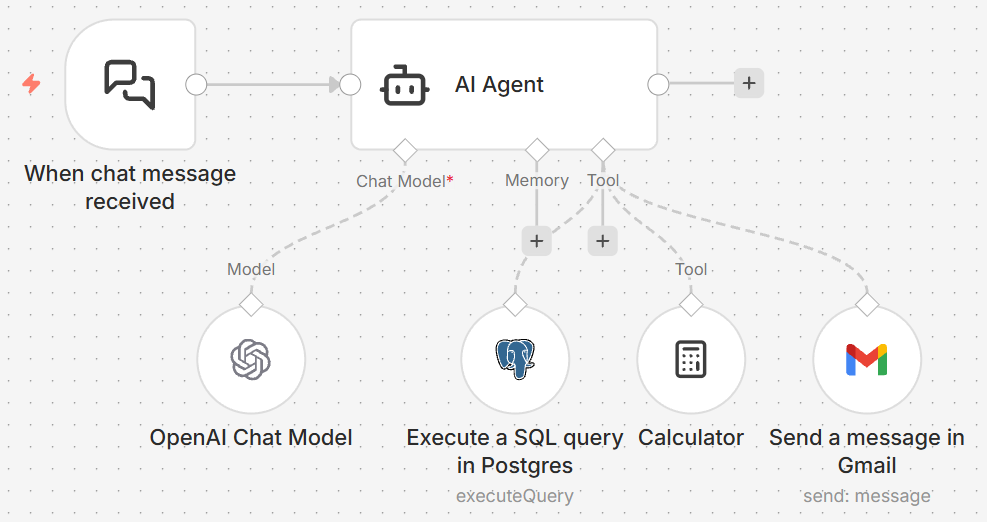
\includegraphics[width=0.65\textwidth]{rysunki/ai_agent.png}
        \captionof{figure}{ Przykład agenta AI wykorzystującego techniką RAG stworzonego z użyciem platformy n8n \cite{n8n}}
        \label{ai_agent}
    \end{center}


        \subsection{Prompt systemowy}
        Prompt systemowy (lub wiadomość systemowa) jest zbiorem instrukcji i kontekstu jaki podaje się do dużego modelu językowego, aby agent AI odpowiadał na pytania w pożądany przez nas sposób. Funkcja ta jest najczęściej wykorzystywana do: 
        \begin{itemize}
            \item ustawienia stylu i tonu odpowiedzi modelu,
            \item zdefiniowania roli i ograniczeń modelu,
            \item określenia kryteriów bezpieczeństwa i jakości podczas generowania odpowiedzi,
            \item wskazania formatu danych wyjściowych (na przykład JSON lub CSV).
        \end{itemize}
